\chapter{Järjestäminen}

\index{järjestäminen}

\key{Järjestäminen}
on keskeinen algoritmiikan ongelma.
Moni tehokas algoritmi
perustuu järjestämiseen,
koska järjestetyn tiedon
käsittely on helpompaa
kuin sekalaisessa järjestyksessä olevan.

Esimerkiksi kysymys ''onko taulukossa kahta samaa
alkiota?'' ratkeaa tehokkaasti järjestämisen avulla.
Jos taulukossa on kaksi samaa alkiota,
ne ovat järjestämisen jälkeen peräkkäin,
jolloin niiden löytäminen on helppoa.
Samaan tapaan ratkeaa myös kysymys
''mikä on yleisin alkio taulukossa?''.

Järjestämiseen on kehitetty monia
algoritmeja, jotka tarjoavat hyviä
esimerkkejä algoritmien suunnittelun tekniikoista.
Tehokkaat yleiset järjestämis\-algoritmit
toimivat ajassa $O(n \log n)$, ja tämä aikavaativuus
on myös monella järjestämistä käyttävällä algoritmilla.

\section{Järjestämisen teoriaa}

Järjestämisen perusongelma on seuraava:

\begin{task}
Annettuna on taulukko, jossa on $n$ alkiota.
Tehtäväsi on järjestää alkiot pienimmästä
suurimpaan.
\end{task}

\noindent
Esimerkiksi taulukko

\begin{center}
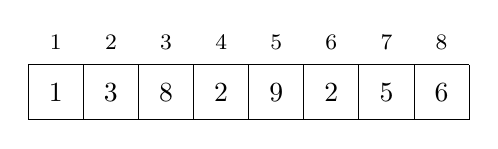
\begin{tikzpicture}[scale=0.7]
\draw (0,0) grid (8,1);
\node at (0.5,0.5) {$1$};
\node at (1.5,0.5) {$3$};
\node at (2.5,0.5) {$8$};
\node at (3.5,0.5) {$2$};
\node at (4.5,0.5) {$9$};
\node at (5.5,0.5) {$2$};
\node at (6.5,0.5) {$5$};
\node at (7.5,0.5) {$6$};

\footnotesize
\node at (0.5,1.4) {$1$};
\node at (1.5,1.4) {$2$};
\node at (2.5,1.4) {$3$};
\node at (3.5,1.4) {$4$};
\node at (4.5,1.4) {$5$};
\node at (5.5,1.4) {$6$};
\node at (6.5,1.4) {$7$};
\node at (7.5,1.4) {$8$};
\end{tikzpicture}
\end{center}

\noindent
on järjestettynä seuraava:

\begin{center}
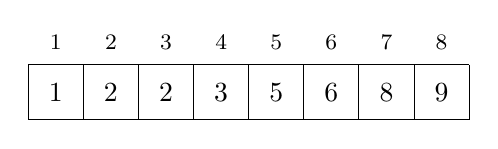
\begin{tikzpicture}[scale=0.7]
\draw (0,0) grid (8,1);
\node at (0.5,0.5) {$1$};
\node at (1.5,0.5) {$2$};
\node at (2.5,0.5) {$2$};
\node at (3.5,0.5) {$3$};
\node at (4.5,0.5) {$5$};
\node at (5.5,0.5) {$6$};
\node at (6.5,0.5) {$8$};
\node at (7.5,0.5) {$9$};

\footnotesize
\node at (0.5,1.4) {$1$};
\node at (1.5,1.4) {$2$};
\node at (2.5,1.4) {$3$};
\node at (3.5,1.4) {$4$};
\node at (4.5,1.4) {$5$};
\node at (5.5,1.4) {$6$};
\node at (6.5,1.4) {$7$};
\node at (7.5,1.4) {$8$};
\end{tikzpicture}
\end{center}

\subsubsection{$O(n^2)$-algoritmit}

\index{kuplajärjestäminen}

Yksinkertaiset algoritmit taulukon
järjestämiseen vievät aikaa $O(n^2)$.
Ehkä tunnetuin tällainen algoritmi on
\key{kuplajärjestäminen} (''bubble sort''),
joka muodostuu peräkkäisistä taulukon läpikäynneistä.

Algoritmissa jokainen taulukon läpikäynti
etsii vierekkäisiä alkiopareja,
jotka ovat väärässä järjestyksessä,
ja korjaa näiden alkioparien järjestyksen.
Algoritmi päättyy, kun läpikäynnin
aikana ei tule mitään muutoksia taulukkoon,
jolloin taulukko on järjestyksessä.

Kuplajärjestämisen voi toteuttaa seuraavasti,
kun järjestettävä taulukko muodostuu alkioista
$\texttt{t}[1],\texttt{t}[2],\ldots,\texttt{t}[n]$:
\begin{lstlisting}
bool stop = false;
while (!stop) {
    stop = true;
    for (int i = 1; i <= n-1; i++) {
        if (t[i] > t[i+1]) {
            swap(t[i],t[i+1]);
            stop = false;
        }
    }
}
\end{lstlisting}

\noindent
Esimerkiksi taulukossa

\begin{center}
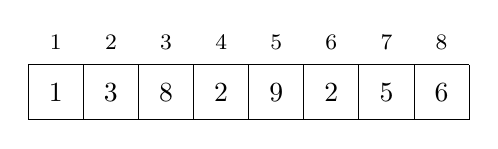
\begin{tikzpicture}[scale=0.7]
\draw (0,0) grid (8,1);

\node at (0.5,0.5) {$1$};
\node at (1.5,0.5) {$3$};
\node at (2.5,0.5) {$8$};
\node at (3.5,0.5) {$2$};
\node at (4.5,0.5) {$9$};
\node at (5.5,0.5) {$2$};
\node at (6.5,0.5) {$5$};
\node at (7.5,0.5) {$6$};

\footnotesize
\node at (0.5,1.4) {$1$};
\node at (1.5,1.4) {$2$};
\node at (2.5,1.4) {$3$};
\node at (3.5,1.4) {$4$};
\node at (4.5,1.4) {$5$};
\node at (5.5,1.4) {$6$};
\node at (6.5,1.4) {$7$};
\node at (7.5,1.4) {$8$};
\end{tikzpicture}
\end{center}

\noindent
kuplajärjestämisen ensimmäinen
läpikäynti tekee seuraavat vaihdot:

\begin{center}
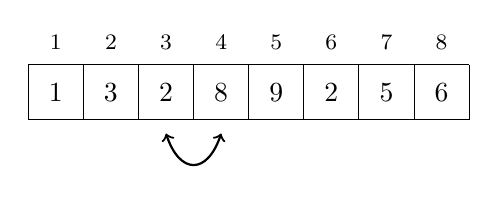
\begin{tikzpicture}[scale=0.7]
\draw (0,0) grid (8,1);
\node at (0.5,0.5) {$1$};
\node at (1.5,0.5) {$3$};
\node at (2.5,0.5) {$2$};
\node at (3.5,0.5) {$8$};
\node at (4.5,0.5) {$9$};
\node at (5.5,0.5) {$2$};
\node at (6.5,0.5) {$5$};
\node at (7.5,0.5) {$6$};

\draw[thick,<->] (3.5,-0.25) .. controls (3.25,-1.00) and (2.75,-1.00) .. (2.5,-0.25);

\footnotesize
\node at (0.5,1.4) {$1$};
\node at (1.5,1.4) {$2$};
\node at (2.5,1.4) {$3$};
\node at (3.5,1.4) {$4$};
\node at (4.5,1.4) {$5$};
\node at (5.5,1.4) {$6$};
\node at (6.5,1.4) {$7$};
\node at (7.5,1.4) {$8$};
\end{tikzpicture}
\end{center}

\begin{center}
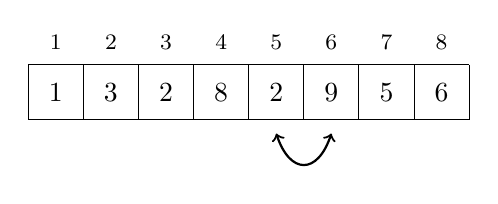
\begin{tikzpicture}[scale=0.7]
\draw (0,0) grid (8,1);
\node at (0.5,0.5) {$1$};
\node at (1.5,0.5) {$3$};
\node at (2.5,0.5) {$2$};
\node at (3.5,0.5) {$8$};
\node at (4.5,0.5) {$2$};
\node at (5.5,0.5) {$9$};
\node at (6.5,0.5) {$5$};
\node at (7.5,0.5) {$6$};

\draw[thick,<->] (5.5,-0.25) .. controls (5.25,-1.00) and (4.75,-1.00) .. (4.5,-0.25);


\footnotesize
\node at (0.5,1.4) {$1$};
\node at (1.5,1.4) {$2$};
\node at (2.5,1.4) {$3$};
\node at (3.5,1.4) {$4$};
\node at (4.5,1.4) {$5$};
\node at (5.5,1.4) {$6$};
\node at (6.5,1.4) {$7$};
\node at (7.5,1.4) {$8$};
\end{tikzpicture}
\end{center}

\begin{center}
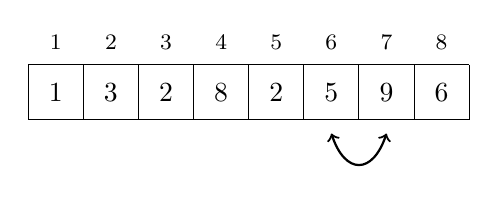
\begin{tikzpicture}[scale=0.7]
\draw (0,0) grid (8,1);
\node at (0.5,0.5) {$1$};
\node at (1.5,0.5) {$3$};
\node at (2.5,0.5) {$2$};
\node at (3.5,0.5) {$8$};
\node at (4.5,0.5) {$2$};
\node at (5.5,0.5) {$5$};
\node at (6.5,0.5) {$9$};
\node at (7.5,0.5) {$6$};

\draw[thick,<->] (6.5,-0.25) .. controls (6.25,-1.00) and (5.75,-1.00) .. (5.5,-0.25);


\footnotesize
\node at (0.5,1.4) {$1$};
\node at (1.5,1.4) {$2$};
\node at (2.5,1.4) {$3$};
\node at (3.5,1.4) {$4$};
\node at (4.5,1.4) {$5$};
\node at (5.5,1.4) {$6$};
\node at (6.5,1.4) {$7$};
\node at (7.5,1.4) {$8$};
\end{tikzpicture}
\end{center}

\begin{center}
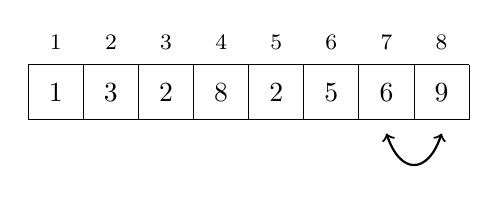
\begin{tikzpicture}[scale=0.7]
\draw (0,0) grid (8,1);
\node at (0.5,0.5) {$1$};
\node at (1.5,0.5) {$3$};
\node at (2.5,0.5) {$2$};
\node at (3.5,0.5) {$8$};
\node at (4.5,0.5) {$2$};
\node at (5.5,0.5) {$5$};
\node at (6.5,0.5) {$6$};
\node at (7.5,0.5) {$9$};

\draw[thick,<->] (7.5,-0.25) .. controls (7.25,-1.00) and (6.75,-1.00) .. (6.5,-0.25);

\footnotesize
\node at (0.5,1.4) {$1$};
\node at (1.5,1.4) {$2$};
\node at (2.5,1.4) {$3$};
\node at (3.5,1.4) {$4$};
\node at (4.5,1.4) {$5$};
\node at (5.5,1.4) {$6$};
\node at (6.5,1.4) {$7$};
\node at (7.5,1.4) {$8$};
\end{tikzpicture}
\end{center}


Kuplajärjestämisessä ensimmäisen läpikäynnin jälkeen suurin alkio
on paikallaan, toisen läpikäynnin jälkeen
kaksi suurinta alkiota on paikallaan, jne.
Niinpä kuplajärjestäminen päättyy aina viimeistään $n$
läpikäynnin jälkeen.
Koska jokainen läpikäynti vie aikaa $O(n)$,
algoritmin aikavaativuus on $O(n^2)$.

\subsubsection{Inversiot}

\index{inversio}

Kuplajärjestäminen on esimerkki algoritmista,
joka perustuu taulukon vierekkäisten alkioiden
vaihtamiseen.
Osoittautuu, että minkään tällaisen algoritmin
aikavaativuus ei voi olla parempi kuin $O(n^2)$,
koska tarvittava vaihtojen määrä
saattaa olla luokkaa $O(n^2)$.

Hyödyllinen käsite järjestämisalgoritmien
analyysissa on \key{inversio}.
Se on indeksipari $(a,b)$, joille $a<b$
ja $\texttt{t}[a]>\texttt{t}[b]$
eli kaksi taulukon alkiota, jotka ovat väärässä
järjestyksessä.
Esimerkiksi taulukossa

\begin{center}
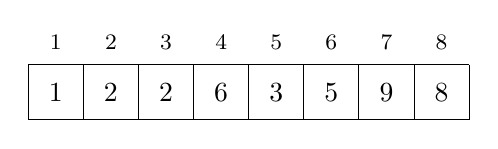
\begin{tikzpicture}[scale=0.7]
\draw (0,0) grid (8,1);
\node at (0.5,0.5) {$1$};
\node at (1.5,0.5) {$2$};
\node at (2.5,0.5) {$2$};
\node at (3.5,0.5) {$6$};
\node at (4.5,0.5) {$3$};
\node at (5.5,0.5) {$5$};
\node at (6.5,0.5) {$9$};
\node at (7.5,0.5) {$8$};

\footnotesize
\node at (0.5,1.4) {$1$};
\node at (1.5,1.4) {$2$};
\node at (2.5,1.4) {$3$};
\node at (3.5,1.4) {$4$};
\node at (4.5,1.4) {$5$};
\node at (5.5,1.4) {$6$};
\node at (6.5,1.4) {$7$};
\node at (7.5,1.4) {$8$};
\end{tikzpicture}
\end{center}

inversiot ovat $(4,5)$, $(4,6)$ ja $(7,8)$.
Inversioiden määrä kuvaa, miten lähellä
järjestystä taulukko on.
Järjestetyn taulukon inversioiden määrä on 0,
ja käänteisesti järjestetyn taulukon
inversioiden määrä on $1+2+\cdots+(n-1)=\frac{n(n-1)}{2}$.

Jos vierekkäiset alkiot ovat väärässä järjestyksessä,
niiden vaihtaminen keskenään poistaa
taulukosta yhden inversion.
Niinpä inversioiden määrä on sama kuin
taulukon järjestämiseen tarvittava vaihtojen määrä.
Vierekkäisiä alkioita
vaihtavan algoritmin aikavaativuus
on aina ainakin $O(n^2)$,
koska sen täytyy tehdä pahimmassa tapauksessa
$\frac{n(n-1)}{2} = O(n^2)$ vaihtoa.

\subsubsection{$O(n \log n)$-algoritmit}

\index{lomitusjärjestäminen}

Tehokkaat järjestämisalgoritmit vievät
aikaa $O(n \log n)$.
Yksi tällainen algoritmi on
\key{lomitusjärjestäminen} (''merge sort''),
joka järjestää taulukon
rekursiivisesti jakamalla sen
pienemmiksi osataulukoiksi.

Lomitusjärjestäminen
jakaa taulukon kahdeksi osataulukoksi,
järjestää osataulukot rekursiivisesti ja muodostaa
sitten järjestetyn taulukon yhdistämällä osataulukot.
Algoritmin runko on seuraava:
\begin{lstlisting}
void mergesort(int a, int b) {
    if (a == b) return;
    int c = (a+b)/2;
    mergesort(a,c);
    mergesort(c+1,b);
    merge(a,c,c+1,b);
}
\end{lstlisting}
Funktio \texttt{mergesort}
järjestää taulukon välin $a \ldots b$ alkiot.
Jos $a=b$, välillä on vain yksi alkio,
joten se on valmiiksi järjestyksessä.
Muuten algoritmi jakaa välin
kahteen osaan: vasen osa on väli $a \ldots c$
ja oikea osa on väli $c+1 \ldots b$, missä $c=(a+b)/2$.
Algoritmi järjestää osat rekursiivisesti
kutsumalla itseään.

Algoritmi kutsuu funktiota \texttt{merge},
joka lomittaa välin vasemman ja oikean osan alkiot.
Tämä tarkoittaa, että alkiot kerätään yhteen niin,
että koko taulukon väli on järjestyksessä.
Lomitus
on mahdollista toteuttaa ajassa $O(n)$
valitsemalla alkiot järjestyksessä vasemman ja
oikean osan alusta alkaen.

\begin{samepage}
Esimerkiksi taulukko

\begin{center}
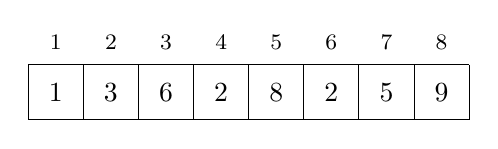
\begin{tikzpicture}[scale=0.7]
\draw (0,0) grid (8,1);
\node at (0.5,0.5) {$1$};
\node at (1.5,0.5) {$3$};
\node at (2.5,0.5) {$6$};
\node at (3.5,0.5) {$2$};
\node at (4.5,0.5) {$8$};
\node at (5.5,0.5) {$2$};
\node at (6.5,0.5) {$5$};
\node at (7.5,0.5) {$9$};

\footnotesize
\node at (0.5,1.4) {$1$};
\node at (1.5,1.4) {$2$};
\node at (2.5,1.4) {$3$};
\node at (3.5,1.4) {$4$};
\node at (4.5,1.4) {$5$};
\node at (5.5,1.4) {$6$};
\node at (6.5,1.4) {$7$};
\node at (7.5,1.4) {$8$};
\end{tikzpicture}
\end{center}
\end{samepage}

jakautuu osataulukoiksi

\begin{center}
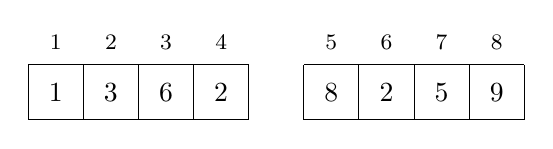
\begin{tikzpicture}[scale=0.7]
\draw (0,0) grid (4,1);
\draw (5,0) grid (9,1);

\node at (0.5,0.5) {$1$};
\node at (1.5,0.5) {$3$};
\node at (2.5,0.5) {$6$};
\node at (3.5,0.5) {$2$};

\node at (5.5,0.5) {$8$};
\node at (6.5,0.5) {$2$};
\node at (7.5,0.5) {$5$};
\node at (8.5,0.5) {$9$};

\footnotesize
\node at (0.5,1.4) {$1$};
\node at (1.5,1.4) {$2$};
\node at (2.5,1.4) {$3$};
\node at (3.5,1.4) {$4$};
\node at (5.5,1.4) {$5$};
\node at (6.5,1.4) {$6$};
\node at (7.5,1.4) {$7$};
\node at (8.5,1.4) {$8$};

\end{tikzpicture}
\end{center}

jotka ovat järjestettyinä:

\begin{center}
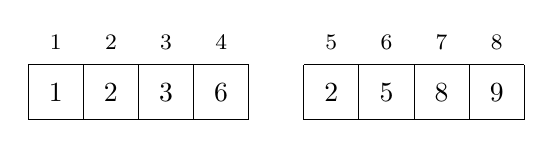
\begin{tikzpicture}[scale=0.7]
\draw (0,0) grid (4,1);
\draw (5,0) grid (9,1);

\node at (0.5,0.5) {$1$};
\node at (1.5,0.5) {$2$};
\node at (2.5,0.5) {$3$};
\node at (3.5,0.5) {$6$};

\node at (5.5,0.5) {$2$};
\node at (6.5,0.5) {$5$};
\node at (7.5,0.5) {$8$};
\node at (8.5,0.5) {$9$};

\footnotesize
\node at (0.5,1.4) {$1$};
\node at (1.5,1.4) {$2$};
\node at (2.5,1.4) {$3$};
\node at (3.5,1.4) {$4$};
\node at (5.5,1.4) {$5$};
\node at (6.5,1.4) {$6$};
\node at (7.5,1.4) {$7$};
\node at (8.5,1.4) {$8$};
\end{tikzpicture}
\end{center}

Osataulukot lomittamalla syntyy järjestetty taulukko

\begin{center}
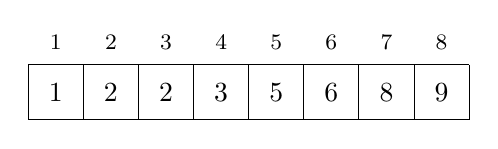
\begin{tikzpicture}[scale=0.7]
\draw (0,0) grid (8,1);
\node at (0.5,0.5) {$1$};
\node at (1.5,0.5) {$2$};
\node at (2.5,0.5) {$2$};
\node at (3.5,0.5) {$3$};
\node at (4.5,0.5) {$5$};
\node at (5.5,0.5) {$6$};
\node at (6.5,0.5) {$8$};
\node at (7.5,0.5) {$9$};

\footnotesize
\node at (0.5,1.4) {$1$};
\node at (1.5,1.4) {$2$};
\node at (2.5,1.4) {$3$};
\node at (3.5,1.4) {$4$};
\node at (4.5,1.4) {$5$};
\node at (5.5,1.4) {$6$};
\node at (6.5,1.4) {$7$};
\node at (7.5,1.4) {$8$};
\end{tikzpicture}
\end{center}

Lomitusjärjestämisen aikavaativuus on $O(n \log n)$,
koska algoritmin aikana
osataulukoista muodostuu $O(\log n)$ tasoa
ja kullakin tasolla osataulukoiden lomitus
vie yhteensä $O(n)$ aikaa.

\subsubsection{Järjestämisen alaraja}

\index{pikajärjestäminen}
\index{kekojärjestäminen}

Monet järjestämisalgoritmi saavuttavat
aikavaativuuden $O(n \log n)$,
mutta kukaan ei ole onnistunut keksimään
yleistä järjestämisalgoritmia,
joka toimisi nopeammin kuin $O(n \log n)$.
Tähän on yllättävä syy: on mahdollista todistaa,
että tällaista algoritmia ei ole olemassa.

Ideana todistuksessa on tarkastella järjestämistä
prosessina, jossa jokainen kahden alkion vertailu
antaa lisää tietoa taulukon sisällöstä.
Prosessista muodostuu seuraavanlainen puu:

\begin{center}
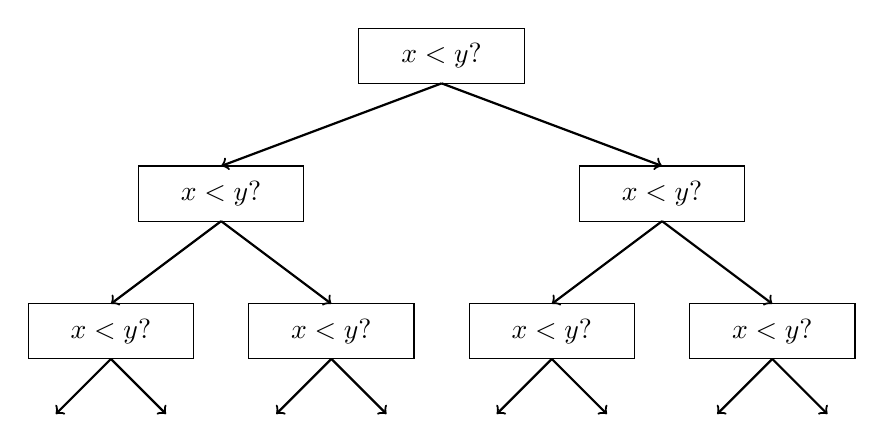
\begin{tikzpicture}[scale=0.7]
\draw (0,0) rectangle (3,1);
\node at (1.5,0.5) {$x < y?$};

\draw[thick,->] (1.5,0) -- (-2.5,-1.5);
\draw[thick,->] (1.5,0) -- (5.5,-1.5);

\draw (-4,-2.5) rectangle (-1,-1.5);
\draw (4,-2.5) rectangle (7,-1.5);
\node at (-2.5,-2) {$x < y?$};
\node at (5.5,-2) {$x < y?$};

\draw[thick,->] (-2.5,-2.5) -- (-4.5,-4);
\draw[thick,->] (-2.5,-2.5) -- (-0.5,-4);
\draw[thick,->] (5.5,-2.5) -- (3.5,-4);
\draw[thick,->] (5.5,-2.5) -- (7.5,-4);

\draw (-6,-5) rectangle (-3,-4);
\draw (-2,-5) rectangle (1,-4);
\draw (2,-5) rectangle (5,-4);
\draw (6,-5) rectangle (9,-4);
\node at (-4.5,-4.5) {$x < y?$};
\node at (-0.5,-4.5) {$x < y?$};
\node at (3.5,-4.5) {$x < y?$};
\node at (7.5,-4.5) {$x < y?$};

\draw[thick,->] (-4.5,-5) -- (-5.5,-6);
\draw[thick,->] (-4.5,-5) -- (-3.5,-6);
\draw[thick,->] (-0.5,-5) -- (0.5,-6);
\draw[thick,->] (-0.5,-5) -- (-1.5,-6);
\draw[thick,->] (3.5,-5) -- (2.5,-6);
\draw[thick,->] (3.5,-5) -- (4.5,-6);
\draw[thick,->] (7.5,-5) -- (6.5,-6);
\draw[thick,->] (7.5,-5) -- (8.5,-6);
\end{tikzpicture}
\end{center}

Merkintä ''$x<y?$'' tarkoittaa taulukon alkioiden
$x$ ja $y$ vertailua.
Jos $x<y$, prosessi jatkaa vasemmalle,
ja muuten oikealle.
Prosessin tulokset ovat taulukon mahdolliset
järjestykset, joita on kaikkiaan $n!$ erilaista.
Puun korkeuden tulee olla tämän vuoksi vähintään

\[ \log_2(n!) = \log_2(1)+\log_2(2)+\cdots+\log_2(n) = O(n \log n).\]

\subsubsection{Laskemisjärjestäminen}

\index{laskemisjärjestäminen}

Järjestämisen alaraja $O(n \log n)$ ei koske algoritmeja,
jotka eivät perustu alkioiden vertailuun vaan hyödyntävät
jotain muuta tietoa alkioista.
Esimerkki tällaisesta algoritmista on
\key{laskemisjärjestäminen}, joka järjestää
kokonaisluvuista koostuvan taulukon $O(n)$-ajassa.

Algoritmin ideana on luoda \emph{kirjanpito}, josta selviää,
montako kertaa mikäkin alkio esiintyy taulukossa.
Kirjanpito on taulukko, jonka indeksit ovat alkuperäisen
taulukon alkioita.
Jokaisen indeksin kohdalla lukee, montako kertaa
kyseinen alkio esiintyy alkuperäisessä taulukossa.

Esimerkiksi taulukosta

\begin{center}
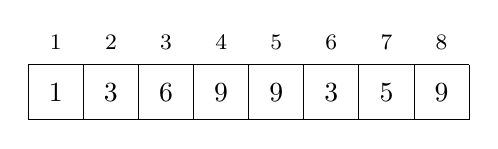
\begin{tikzpicture}[scale=0.7]
\draw (0,0) grid (8,1);
\node at (0.5,0.5) {$1$};
\node at (1.5,0.5) {$3$};
\node at (2.5,0.5) {$6$};
\node at (3.5,0.5) {$9$};
\node at (4.5,0.5) {$9$};
\node at (5.5,0.5) {$3$};
\node at (6.5,0.5) {$5$};
\node at (7.5,0.5) {$9$};

\footnotesize
\node at (0.5,1.4) {$1$};
\node at (1.5,1.4) {$2$};
\node at (2.5,1.4) {$3$};
\node at (3.5,1.4) {$4$};
\node at (4.5,1.4) {$5$};
\node at (5.5,1.4) {$6$};
\node at (6.5,1.4) {$7$};
\node at (7.5,1.4) {$8$};
\end{tikzpicture}
\end{center}

syntyy seuraava kirjanpito:

\begin{center}
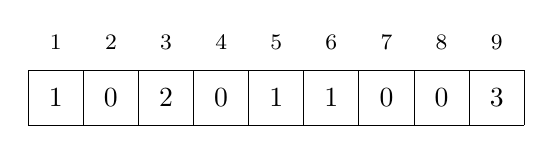
\begin{tikzpicture}[scale=0.7]
\draw (0,0) grid (9,1);
\node at (0.5,0.5) {$1$};
\node at (1.5,0.5) {$0$};
\node at (2.5,0.5) {$2$};
\node at (3.5,0.5) {$0$};
\node at (4.5,0.5) {$1$};
\node at (5.5,0.5) {$1$};
\node at (6.5,0.5) {$0$};
\node at (7.5,0.5) {$0$};
\node at (8.5,0.5) {$3$};

\footnotesize

\node at (0.5,1.5) {$1$};
\node at (1.5,1.5) {$2$};
\node at (2.5,1.5) {$3$};
\node at (3.5,1.5) {$4$};
\node at (4.5,1.5) {$5$};
\node at (5.5,1.5) {$6$};
\node at (6.5,1.5) {$7$};
\node at (7.5,1.5) {$8$};
\node at (8.5,1.5) {$9$};
\end{tikzpicture}
\end{center}

Esimerkiksi kirjanpidossa lukee indeksin 3 kohdalla 2,
koska luku 3 esiintyy kahdesti alkuperäisessä
taulukossa (indekseissä 2 ja 6).

Kirjanpidon muodostus vie aikaa $O(n)$,
koska riittää käydä taulukko läpi kerran.
Tämän jälkeen järjestetyn taulukon luominen
vie myös aikaa $O(n)$, koska kunkin alkion
määrän saa selville suoraan kirjanpidosta.
Niinpä laskemisjärjestämisen
kokonaisaikavaativuus on $O(n)$.

Laskemisjärjestäminen on hyvin tehokas algoritmi,
mutta sen käyttäminen vaatii,
että taulukon sisältönä on niin pieniä
kokonaislukuja, että niitä voi käyttää
kirjanpidon taulukon indeksöinnissä.

\section{Järjestäminen C++:ssa}

\index{\texttt{sort}}

C++:n standardikirjastossa on funktio \texttt{sort},
jonka avulla voi järjestää helposti taulukoita
ja muita tietorakenteita.
Tätä funktiota kannattaa käyttää yleensä aina
järjestämiseen algoritmeissa,
koska funktio on toteutettu tehokkaasti ja varmasti toimivasti.

\begin{minipage}{\textwidth}
Seuraava koodi järjestää vektorin \texttt{v}
luvut pienimmästä suurimpaan:

\begin{lstlisting}
vector<int> v = {4,2,5,3,5,8,3};
sort(v.begin(),v.end());
\end{lstlisting}
\end{minipage}

Järjestämisen jälkeen vektorin sisältö on
$\{2,3,3,4,5,5,8\}$.

Oletuksena järjestys tapahtuu pienimmästä suurimpaan,
mutta järjestyksen saa käänteiseksi näin:

\begin{lstlisting}
sort(v.rbegin(),v.rend());
\end{lstlisting}

Tavallisen taulukon voi järjestää seuraavasti:

\begin{lstlisting}
int n = 7; // taulukon koko
int t[] = {4,2,5,3,5,8,3};
sort(t,t+n);
\end{lstlisting}

Seuraava koodi järjestää merkkijonon \texttt{s}:

\begin{lstlisting}
string s = "apina";
sort(s.begin(), s.end());
\end{lstlisting}

Merkkijonon järjestäminen tarkoittaa,
että sen merkit järjestetään aakkosjärjestykseen.
Esimerkiksi merkkijono ''apina''
on järjestettynä ''aainp''.

\subsubsection{Vertailuoperaattori}

\index{vertailuoperaattori}

Funktion \texttt{sort} käyttäminen vaatii,
että järjestettävien alkioiden
tietotyypille on määritelty \key{vertailuoperaattori} \texttt{<},
jonka avulla voi selvittää, mikä on kahden alkion järjestys.
Järjestämisen aikana \texttt{sort}-funktio
käyttää operaattoria \texttt{<} aina, kun sen täytyy
vertailla järjestettäviä alkioita.

Vertailuoperaattori on määritelty valmiiksi
useimmille C++:n tietotyypeille,
minkä ansiosta niitä pystyy järjestämään automaattisesti.
Jos järjestettävänä on lukuja, ne järjestyvät
suuruusjärjestykseen,
ja jos järjestettävänä on merkkijonoja,
ne järjestyvät aakkosjärjestykseen.

Parit (\texttt{pair}) järjestyvät ensisijaisesti
ensimmäisen kentän (\texttt{first}) mukaan.
Jos kuitenkin parien ensimmäiset kentät ovat samat,
järjestys määräytyy toisen kentän (\texttt{second}) mukaan.
Seuraava koodi esittelee asiaa:

\begin{lstlisting}
vector<pair<int,int>> v;
v.push_back({1,5});
v.push_back({2,3});
v.push_back({1,2});
sort(v.begin(), v.end());
\end{lstlisting}

Koodin suorituksen jälkeen parien järjestys on
$(1,2)$, $(1,5)$, $(2,3)$.

Jos järjestettävänä on omia tietueita,
niiden vertailuoperaattori täytyy toteuttaa itse.
Operaattori määritellään tietueen sisään
\texttt{operator<}-nimisenä funktiona,
jonka parametrina on toinen alkio.
Operaattorin tulee palauttaa \texttt{true},
jos oma alkio on pienempi kuin parametrialkio,
ja muuten \texttt{false}.

Esimerkiksi seuraava tietue \texttt{P}
sisältää pisteen x- ja y-koordinaatit.
Vertailuoperaattori on toteutettu niin,
että pisteet järjestyvät ensisijaisesti x-koor\-di\-naa\-tin
ja toissijaisesti y-koordinaatin mukaan.

\begin{lstlisting}
struct P {
    int x, y;
    bool operator<(const p& a) {
        if (this.x != a.x) return this.x < a.x;
        else return this.y < a.y;
    }
};
\end{lstlisting}

\subsubsection{Vertailufunktio}

\index{vertailufunktio}

On myös mahdollista antaa
\texttt{sort}-funktiolle ulkopuolinen \key{vertailufunktio}.
Esimerkiksi seuraava vertailufunktio
järjestää merkkijonot ensisijaisesti pituuden mukaan
ja toissijaisesti aakkosjärjestyksen mukaan:

\begin{lstlisting}
bool cmp(string a, string b) {
    if (a.size() != b.size()) return a.size() < b.size();
    return a < b;
}
\end{lstlisting}

Tämän jälkeen merkkijonovektorin voi järjestää näin:

\begin{lstlisting}
sort(v.begin(), v.end(), cmp);
\end{lstlisting}

\section{Binäärihaku}

\index{binäärihaku}

Tavallinen tapa etsiä alkiota $x$ taulukosta \texttt{t}
on käyttää \texttt{for}-silmukkaa, joka käy läpi
taulukon sisällön:

\begin{lstlisting}
for (int i = 1; i <= n; i++) {
    if (t[i] == x) // alkio x löytyi kohdasta i
}
\end{lstlisting}

Tämän menetelmän aikavaativuus on $O(n)$,
koska pahimmassa tapauksessa koko taulukko täytyy
käydä läpi.
Jos taulukon sisältö voi olla mitä tahansa,
tämä on kuitenkin tehokkain mahdollinen menetelmä,
koska saatavilla ei ole lisätietoa siitä,
mistä päin taulukkoa alkiota $x$ kannattaa etsiä.

Tilanne on toinen silloin, kun taulukko on
järjestyksessä.
Tässä tapauksessa haku on mahdollista toteuttaa
paljon nopeammin, koska alkioiden järjestys
ohjaa etsimään alkiota oikeasta suunnasta.
Seuraavaksi käsiteltävä \key{binäärihaku}
löytää alkion järjestetystä taulukosta
tehokkaasti ajassa $O(\log n)$.

\subsubsection{Toteutus 1}

Perinteinen tapa toteuttaa binäärihaku muistuttaa sanan etsimistä
sanakirjasta. Haku puolittaa joka askeleella hakualueen taulukossa,
kunnes lopulta etsittävä alkio löytyy tai osoittautuu,
että sitä ei ole taulukossa.

Haku tarkistaa ensin taulukon keskimmäisen alkion.
Jos keskimmäinen alkio on etsittävä alkio, haku päättyy.
Muuten haku jatkuu taulukon vasempaan tai oikeaan osaan sen mukaan,
onko keskimmäinen alkio suurempi vain pienempi kuin etsittävä alkio.

Yllä olevan idean voi toteuttaa seuraavasti:
\begin{lstlisting}
int a = 1, b = n;
while (a <= b) {
    int k = (a+b)/2;
    if (t[k] == x) // alkio x löytyi kohdasta k
    if (t[k] > x) b = k-1;
    else a = k+1;
}
\end{lstlisting}

Algoritmi pitää yllä väliä $a \ldots b$, joka on
jäljellä oleva hakualue taulukossa.
Aluksi väli on $1 \ldots n$ eli koko taulukko.
Välin koko puolittuu algoritmin joka vaiheessa,
joten aikavaativuus on $O(\log n)$.

\subsubsection{Toteutus 2}

Vaihtoehtoinen tapa toteuttaa binäärihaku
perustuu taulukon tehostettuun läpikäyntiin.
Ideana on käydä taulukkoa läpi hyppien
ja hidastaa vauhtia, kun etsittävä alkio lähestyy.

Haku käy taulukkoa läpi vasemmalta oikealle aloittaen
hypyn pituudesta $n$.
Joka vaiheessa hypyn pituus puolittuu:
ensin $n/2$, sitten $n/4$, sitten $n/8$ jne.,
kunnes lopulta hypyn pituus on 1.
Hyppyjen jälkeen joko haettava alkio on löytynyt
tai selviää, että sitä ei ole taulukossa.

Seuraava koodi toteuttaa äskeisen idean:
\begin{lstlisting}
int k = 1;
for (int b = n; b >= 1; b /= 2) {
    while (k+b <= n && t[k+b] <= x) k += b;
}
if (t[k] == x) // alkio x löytyi kohdasta k
\end{lstlisting}

Muuttuja $k$ on läpikäynnin kohta taulukossa
ja muuttuja $b$ on hypyn pituus.
Jos alkio $x$ esiintyy taulukossa,
sen kohta on muuttujassa $k$ algoritmin päätteeksi.
Algoritmin aikavaativuus on $O(\log n)$,
koska \texttt{while}-silmukassa oleva koodi suoritetaan
aina enintään kahdesti.

\subsubsection{Muutoskohdan etsiminen}

Käytännössä binäärihakua tarvitsee koodata
harvoin alkion etsimiseen taulukosta,
koska sen sijasta voi käyttää standardikirjastoa.
Esimerkiksi C++:n funktiot \texttt{lower\_bound}
ja \texttt{upper\_bound} toteuttavat binäärihaun
ja tietorakenne \texttt{set} ylläpitää joukkoa,
jonka operaatiot ovat $O(\log n)$-aikaisia.

Sitäkin tärkeämpi binäärihaun käyttökohde on 
funktion muutoskohdan etsiminen.
Oletetaan, että haluamme löytää pienimmän arvon $k$,
joka on kelvollinen ratkaisu ongelmaan.
Käytössämme on funktio $\texttt{ok}(x)$,
joka palauttaa \texttt{true}, jos $x$ on kelvollinen
ratkaisu, ja muuten \texttt{false}.
Lisäksi tiedämme, että $\texttt{ok}(x)$ on \texttt{false}
aina kun $x<k$ ja \texttt{true} aina kun $x \geq k$.

Toisin sanoen haluamme löytää funktion \texttt{ok} muutoskohdan,
jossa arvosta \texttt{false} tulee arvo \texttt{true}.
Tilanne näyttää seuraavalta:

\begin{center}
\begin{tabular}{r|rrrrrrrr}
$x$ & 0 & 1 & $\cdots$ & $k-1$ & $k$ & $k+1$ & $\cdots$ \\
\hline
$\texttt{ok}(x)$ & \texttt{false} & \texttt{false}
& $\cdots$ & \texttt{false} & \texttt{true} & \texttt{true} & $\cdots$ \\
\end{tabular}
\end{center}

\noindent
Nyt muutoskohta on mahdollista etsiä käyttämällä
binäärihakua:

\begin{lstlisting}
int x = -1;
for (int b = z; b >= 1; b /= 2) {
    while (!ok(x+b)) x += b;
}
int k = x+1;
\end{lstlisting}

Haku etsii suurimman $x$:n arvon,
jolla $\texttt{ok}(x)$ on \texttt{false}.
Niinpä tästä seuraava arvo $k=x+1$
on pienin arvo, jolla $\texttt{ok}(k)$ on \texttt{true}.
Hypyn aloituspituus $z$ tulee olla 
sopiva suuri luku, esimerkiksi sellainen,
jolla $\texttt{ok}(z)$ on varmasti \texttt{true}.

Algoritmi kutsuu $O(\log z)$ kertaa funktiota
\texttt{ok}, joten kokonaisaikavaativuus
riippuu siitä, kauanko funktion \texttt{ok}
suoritus kestää.
Esimerkiksi jos ratkaisun tarkastus
vie aikaa $O(n)$, niin kokonaisaikavaativuus
on $O(n \log z)$.

\subsubsection{Huippuarvon etsiminen}

Binäärihaulla voi myös etsiä
suurimman arvon funktiolle,
joka on ensin kasvava ja sitten laskeva.
Toisin sanoen tehtävänä on etsiä arvo
$k$ niin, että

\begin{itemize}
\item
$f(x)<f(x+1)$, kun $x<k$, ja
\item
$f(x)>f(x+1)$, kun $x >= k$.
\end{itemize}

Ideana on etsiä binäärihaulla
viimeinen kohta $x$,
jossa pätee $f(x)<f(x+1)$.
Tällöin $k=x+1$,
koska pätee $f(x+1)>f(x+2)$.
Seuraava koodi toteuttaa haun: 

\begin{lstlisting}
int x = -1;
for (int b = z; b >= 1; b /= 2) {
    while (f(x+b) < f(x+b+1)) x += b;
}
int k = x+1;
\end{lstlisting}

Huomaa, että toisin kuin tavallisessa binäärihaussa,
tässä ei ole sallittua,
että peräkkäiset arvot olisivat yhtä suuria.
Silloin ei olisi mahdollista tietää,
mihin suuntaan hakua tulee jatkaa.

